\documentclass[handout, 11pt]{beamer}
\mode
<presentation>{\usetheme{Madrid}}
\institute[UF]{\inst{1}
University of Florida\\
Department of Finance, Insurance, and Real Estate}
\usepackage{adjustbox}
\usepackage{tikz}
\usetikzlibrary{positioning}
\usetikzlibrary{positioning}
\usetikzlibrary{positioning}
\usetikzlibrary{positioning}
\usetikzlibrary{positioning}
\usetikzlibrary{positioning}
\usetikzlibrary{positioning}
\usetikzlibrary{positioning}
\usetikzlibrary{positioning}
\usetikzlibrary{positioning}
\usetikzlibrary{positioning}
\usetikzlibrary{positioning}
\usetikzlibrary{positioning}
\usetikzlibrary{positioning}
\usepackage{xcolor}
\setbeamertemplate{headline}{\begin{beamercolorbox}[ht=2.25ex, dp=3.75ex]{section in head/foot}
\insertnavigation{\paperwidth}
\end{beamercolorbox}}
\AtBeginSection{\begin{frame}
\frametitle{Table of Contents}
\tableofcontents[currentsection]
\end{frame}}
\begin{document}
\title[Intro]{Financial Modeling with Python and Excel}
\subtitle{An Introduction}
\author[DeRobertis]{Nick DeRobertis\inst{1}}
\date{\today}
\begin{frame}
\titlepage
\label{title-frame}
\end{frame}
\begin{section}[Intro]{Introduction to Financial Modeling}
\begin{frame}
\frametitle{What is this Class?}
\begin{columns}
\begin{column}{0.5\textwidth}
\vbox to 0.8\textheight{\begin{itemize}
\item This is a skills-based course focused on teaching financial modeling techniques in Python and Excel
\vfill
\item The focus is not a lot of specific models, but rather general model-building techniques
\vfill
\item The focus will be simple models, but extending them in powerful ways
\end{itemize}}
\end{column}
\begin{column}{0.5\textwidth}
\vbox to 0.8\textheight{\centering
\vfill

\includegraphics[height=0.4\textheight, keepaspectratio, width=0.9\textwidth]{Sources/python-logo.png}
\vfill

\includegraphics[height=0.4\textheight, keepaspectratio, width=0.9\textwidth]{Sources/excel-logo.png}
\vfill
\vfill}
\end{column}
\end{columns}
\end{frame}
\begin{frame}
\frametitle{What is a Model?}
\begin{center}
\begin{adjustbox}{width=0.9\textwidth, height=0.8\textheight, keepaspectratio}
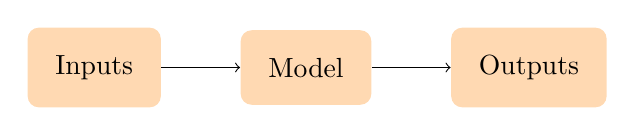
\begin{tikzpicture}
\node [fill=orange!30, rounded corners, inner sep=10pt] (c76dabc2-1964-4a10-b72a-88fafa6f2138)  {Inputs};
\node [fill=orange!30, rounded corners, inner sep=10pt, right=of c76dabc2-1964-4a10-b72a-88fafa6f2138] (ab3d5dad-7dfb-43ae-aa5d-3acc752e0aad)  {Model};
\node [fill=orange!30, rounded corners, inner sep=10pt, right=of ab3d5dad-7dfb-43ae-aa5d-3acc752e0aad] (f9bf7c24-76fd-46b5-aab1-e33305c3d589)  {Outputs};
\path [draw, ->] (c76dabc2-1964-4a10-b72a-88fafa6f2138) -- (ab3d5dad-7dfb-43ae-aa5d-3acc752e0aad);
\path [draw, ->] (ab3d5dad-7dfb-43ae-aa5d-3acc752e0aad) -- (f9bf7c24-76fd-46b5-aab1-e33305c3d589);
\end{tikzpicture}
\end{adjustbox}
\end{center}
\end{frame}
\begin{frame}
\frametitle{A Retirement Problem}
\vspace{-0.25cm}
\begin{block}<+->{A General Structure}
\begin{center}
\begin{adjustbox}{width=0.9\textwidth, height=0.8\textheight, keepaspectratio}
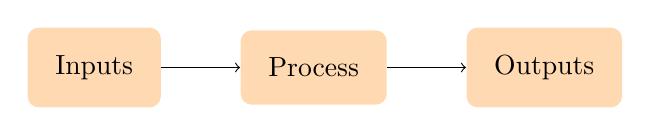
\begin{tikzpicture}
\node [fill=orange!30, rounded corners, inner sep=10pt] (755d7c98-4778-44f2-bbf4-030d2473a6b6)  {Inputs};
\node [fill=orange!30, rounded corners, inner sep=10pt, right=of 755d7c98-4778-44f2-bbf4-030d2473a6b6] (133a4ad1-cb06-49dc-9e20-34fbe122a1bf)  {Process};
\node [fill=orange!30, rounded corners, inner sep=10pt, right=of 133a4ad1-cb06-49dc-9e20-34fbe122a1bf] (80db54e7-5856-4ac2-83b1-7aaf33e6df66)  {Outputs};
\path [draw, ->] (755d7c98-4778-44f2-bbf4-030d2473a6b6) -- (133a4ad1-cb06-49dc-9e20-34fbe122a1bf);
\path [draw, ->] (133a4ad1-cb06-49dc-9e20-34fbe122a1bf) -- (80db54e7-5856-4ac2-83b1-7aaf33e6df66);
\end{tikzpicture}
\end{adjustbox}
\end{center}
\end{block}
\vspace{-0.25cm}
\begin{block}<+->{Real-world Problem}
\begin{center}
\begin{adjustbox}{width=0.9\textwidth, height=0.8\textheight, keepaspectratio}
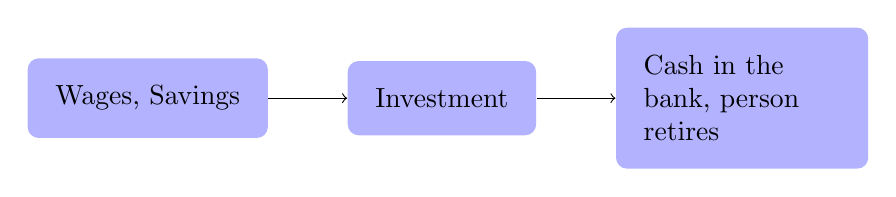
\begin{tikzpicture}
\node [fill=blue!30, rounded corners, inner sep=10pt] (c112de39-eed3-4d4d-a44c-c4ed6acd5201)  {Wages, Savings};
\node [fill=blue!30, rounded corners, inner sep=10pt, right=of c112de39-eed3-4d4d-a44c-c4ed6acd5201] (8fe197b4-2a19-4c68-b29d-77606584eb06)  {Investment};
\node [fill=blue!30, rounded corners, inner sep=10pt, text width=2.5cm, right=of 8fe197b4-2a19-4c68-b29d-77606584eb06] (77b7cfc5-f237-4b8b-ade6-b2b41b402949)  {Cash in the bank, person retires};
\path [draw, ->] (c112de39-eed3-4d4d-a44c-c4ed6acd5201) -- (8fe197b4-2a19-4c68-b29d-77606584eb06);
\path [draw, ->] (8fe197b4-2a19-4c68-b29d-77606584eb06) -- (77b7cfc5-f237-4b8b-ade6-b2b41b402949);
\end{tikzpicture}
\end{adjustbox}
\end{center}
\end{block}
\vspace{-0.25cm}
\begin{block}<+->{A Model of the Problem}
\begin{center}
\begin{adjustbox}{width=0.9\textwidth, height=0.8\textheight, keepaspectratio}
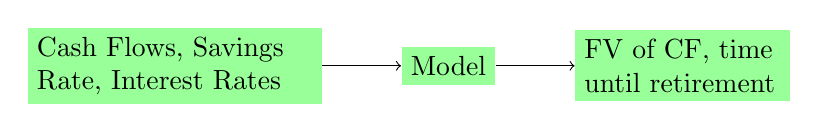
\begin{tikzpicture}
\node [fill=green!40, text width=3.5cm] (170050d0-04a2-4a41-8a84-c7c58c1e31e8)  {Cash Flows, Savings Rate, Interest Rates};
\node [fill=green!40, right=of 170050d0-04a2-4a41-8a84-c7c58c1e31e8] (fc4cf0e5-0c0b-4c33-b31a-5733e1241913)  {Model};
\node [fill=green!40, text width=2.5cm, right=of fc4cf0e5-0c0b-4c33-b31a-5733e1241913] (4a6151fc-a83a-4b5b-9e7c-e5ffde1e4b60)  {FV of CF, time until retirement};
\path [draw, ->] (170050d0-04a2-4a41-8a84-c7c58c1e31e8) -- (fc4cf0e5-0c0b-4c33-b31a-5733e1241913);
\path [draw, ->] (fc4cf0e5-0c0b-4c33-b31a-5733e1241913) -- (4a6151fc-a83a-4b5b-9e7c-e5ffde1e4b60);
\end{tikzpicture}
\end{adjustbox}
\end{center}
\end{block}
\end{frame}
\begin{frame}
\frametitle{Valuing a Company (DCF Model)}
\vspace{-0.25cm}
\begin{block}<+->{A General Structure}
\begin{center}
\begin{adjustbox}{width=0.9\textwidth, height=0.8\textheight, keepaspectratio}
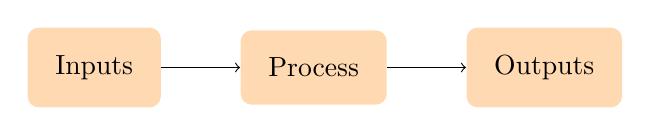
\begin{tikzpicture}
\node [fill=orange!30, rounded corners, inner sep=10pt] (e3ecad63-11ff-437b-bf47-b7a337066c1a)  {Inputs};
\node [fill=orange!30, rounded corners, inner sep=10pt, right=of e3ecad63-11ff-437b-bf47-b7a337066c1a] (dde1cb4a-3654-423a-9639-0239efc395c9)  {Process};
\node [fill=orange!30, rounded corners, inner sep=10pt, right=of dde1cb4a-3654-423a-9639-0239efc395c9] (bd9a2309-8b7f-4c79-a6df-f8a69e27b9b5)  {Outputs};
\path [draw, ->] (e3ecad63-11ff-437b-bf47-b7a337066c1a) -- (dde1cb4a-3654-423a-9639-0239efc395c9);
\path [draw, ->] (dde1cb4a-3654-423a-9639-0239efc395c9) -- (bd9a2309-8b7f-4c79-a6df-f8a69e27b9b5);
\end{tikzpicture}
\end{adjustbox}
\end{center}
\end{block}
\vspace{-0.25cm}
\begin{block}<+->{Real-world Problem}
\begin{center}
\begin{adjustbox}{width=0.9\textwidth, height=0.8\textheight, keepaspectratio}
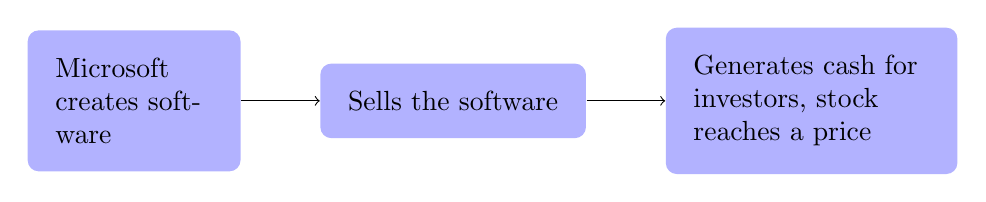
\begin{tikzpicture}
\node [fill=blue!30, rounded corners, inner sep=10pt, text width=2cm] (228c44fd-358e-471a-ba35-a10d2827c4bf)  {Microsoft creates software};
\node [fill=blue!30, rounded corners, inner sep=10pt, right=of 228c44fd-358e-471a-ba35-a10d2827c4bf] (b160c36c-329a-4adb-bc57-1b415066e852)  {Sells the software};
\node [fill=blue!30, rounded corners, inner sep=10pt, text width=3cm, right=of b160c36c-329a-4adb-bc57-1b415066e852] (ec5d97db-2b15-4d47-b739-37459c049e05)  {Generates cash for investors, stock reaches a price};
\path [draw, ->] (228c44fd-358e-471a-ba35-a10d2827c4bf) -- (b160c36c-329a-4adb-bc57-1b415066e852);
\path [draw, ->] (b160c36c-329a-4adb-bc57-1b415066e852) -- (ec5d97db-2b15-4d47-b739-37459c049e05);
\end{tikzpicture}
\end{adjustbox}
\end{center}
\end{block}
\vspace{-0.25cm}
\begin{block}<+->{A Model of the Problem}
\begin{center}
\begin{adjustbox}{width=0.9\textwidth, height=0.8\textheight, keepaspectratio}
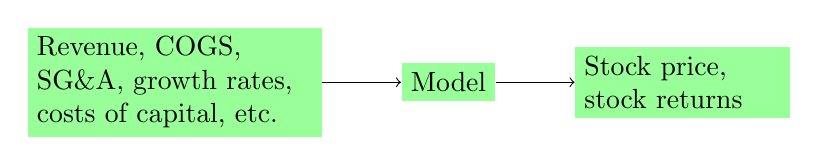
\begin{tikzpicture}
\node [fill=green!40, text width=3.5cm] (3cc024c3-c59c-4785-b03b-7a2ac843d684)  {Revenue, COGS, SG\&A, growth rates, costs of capital, etc.};
\node [fill=green!40, right=of 3cc024c3-c59c-4785-b03b-7a2ac843d684] (f0c47c6f-9d36-4e24-8abc-a56c481fc342)  {Model};
\node [fill=green!40, text width=2.5cm, right=of f0c47c6f-9d36-4e24-8abc-a56c481fc342] (68b4c6ee-00a7-40d9-88fe-fb75febf9b0f)  {Stock price, stock returns};
\path [draw, ->] (3cc024c3-c59c-4785-b03b-7a2ac843d684) -- (f0c47c6f-9d36-4e24-8abc-a56c481fc342);
\path [draw, ->] (f0c47c6f-9d36-4e24-8abc-a56c481fc342) -- (68b4c6ee-00a7-40d9-88fe-fb75febf9b0f);
\end{tikzpicture}
\end{adjustbox}
\end{center}
\end{block}
\end{frame}
\end{section}
\begin{section}[Tools and Skills]{Introduction to the Modeling Toolset}
\begin{frame}
\frametitle{Why Python?}
\begin{center}
\begin{adjustbox}{width=0.9\textwidth, height=0.8\textheight, keepaspectratio}
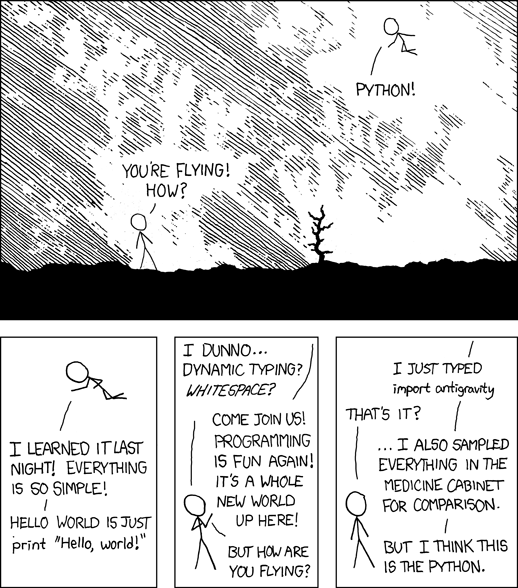
\includegraphics[width=1.0\textwidth]{Sources/xkcd-python.png}
\end{adjustbox}
\end{center}
\end{frame}
\begin{frame}
\frametitle{Python is a Good Choice for Finance}
\begin{itemize}
\item The easiest to learn mainstream programming language
\vfill
\item Heavily used in the financial industry
\end{itemize}
\vfill
\begin{block}<+>{Python is the Most Flexible of the Top Languages}
\begin{columns}
\begin{column}{0.45\textwidth}
\begin{itemize}
\item Modeling
\item Data science
\item Algorithmic Trading
\item Scripting
\end{itemize}
\end{column}
\begin{column}{0.45\textwidth}
\begin{itemize}
\item Devices
\item Web Development
\item Web Scraping
\item Even these slides
\end{itemize}
\end{column}
\end{columns}
\end{block}
\end{frame}
\begin{frame}
\frametitle{Python is the Fastest Growing Programming Lanugage}
\begin{center}
\begin{adjustbox}{width=0.9\textwidth, height=0.8\textheight, keepaspectratio}
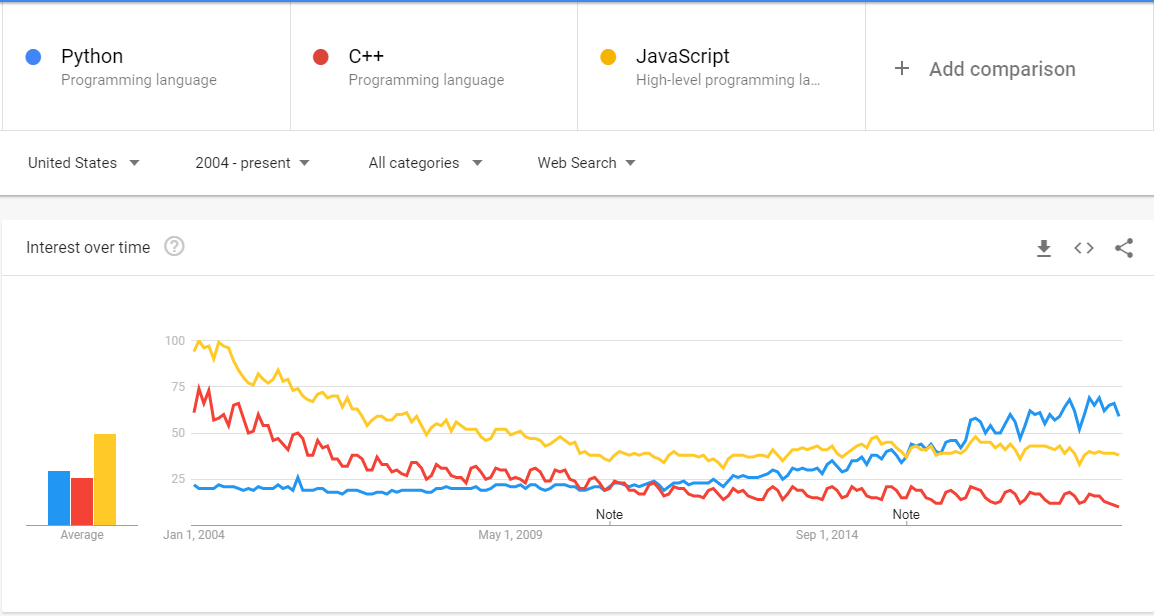
\includegraphics[width=1.0\textwidth]{Sources/python-popularity.PNG}
\end{adjustbox}
\end{center}
\end{frame}
\begin{frame}
\frametitle{More Python Advantages}
\begin{itemize}
\item Open source - completely free and open
\vfill
\item Focus on readability - almost pseudo-code
\vfill
\item Take as much as you need. Easy for beginners, many features for experts.
\vfill
\item Deep integrations with Excel - VBA replacement, run Python in Excel, run Excel from Python
\end{itemize}
\end{frame}
\begin{frame}
\frametitle{Why Not use Python?}
\begin{center}
\begin{adjustbox}{width=0.9\textwidth, height=0.8\textheight, keepaspectratio}
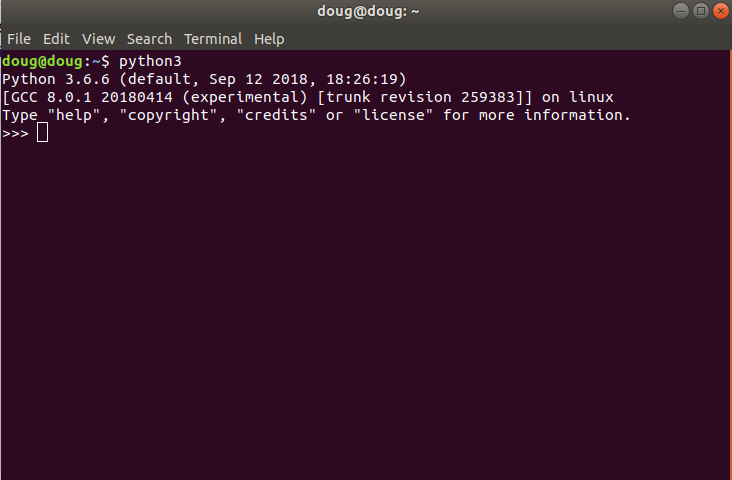
\includegraphics[width=1.0\textwidth]{Sources/python-terminal.png}
\end{adjustbox}
\end{center}
\end{frame}
\begin{frame}
\frametitle{Python Disadvantages}
\begin{itemize}
\item No graphical interface (by default)
\vfill
\item Hard to get others working with it if they don't know Python
\vfill
\item Can take more work to get started on a project
\end{itemize}
\end{frame}
\begin{frame}
\frametitle{Why Not use VBA?}
\begin{center}
\begin{adjustbox}{width=0.9\textwidth, height=0.8\textheight, keepaspectratio}
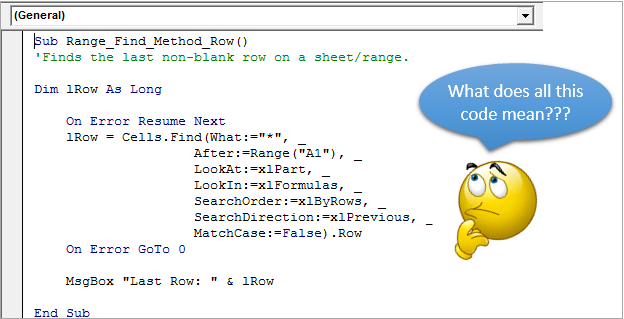
\includegraphics[width=1.0\textwidth]{Sources/vba-terminal.png}
\end{adjustbox}
\end{center}
\end{frame}
\begin{frame}
\frametitle{VBA is Old-School}
\begin{columns}
\begin{column}{0.5\textwidth}
\vbox to 0.8\textheight{\begin{itemize}
\item Code is not as readable as Python
\vfill
\item Power is limited to working within Microsoft Office
\vfill
\item Python has a complete VBA API built into a package - Python can do VBA and more
\end{itemize}}
\end{column}
\begin{column}{0.5\textwidth}
\vbox to 0.8\textheight{\centering
\vfill

\includegraphics[height=1.0\textheight, keepaspectratio, width=0.9\textwidth]{Sources/vba-logo.png}
\vfill
\vfill}
\end{column}
\end{columns}
\end{frame}
\begin{frame}
\frametitle{We Can't Ditch Excel Yet}
\begin{itemize}
\item Excel is everywhere. Most of the world's data is in Excel spreadsheets
\vfill
\item (Nearly) everyone knows how use it
\vfill
\item You can see what you're doing (without effort)
\vfill
\item Easy introspection into a particular value
\end{itemize}
\end{frame}
\begin{frame}
\frametitle{Escaping Excel Hell}
\begin{center}
\begin{adjustbox}{width=0.9\textwidth, height=0.8\textheight, keepaspectratio}
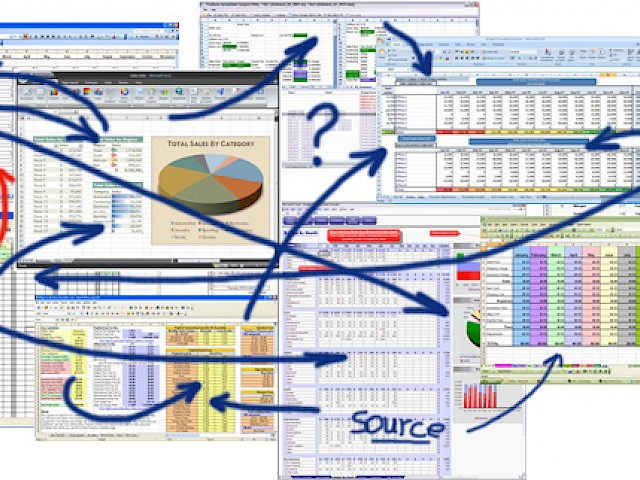
\includegraphics[width=1.0\textwidth]{Sources/excel-hell.jpg}
\end{adjustbox}
\end{center}
\end{frame}
\begin{frame}
\frametitle{The Pains of Excel}
\begin{itemize}
\item Code and view are mixed together, code is hidden
\vfill
\item Both cell formulas and VBA macros - What is going on?
\vfill
\item Easy to make mistakes (one cell different)
\vfill
\item Some tasks which are very simple in Python are very complex in Excel
\end{itemize}
\end{frame}
\begin{frame}
\frametitle{Let's Get Python Set Up on your System}
{
\setbeamercolor{block title}{bg=violet}
\begin{block}{Install Steps}
\small
\begin{enumerate}
\item Go to \textcolor{blue}{\underline{\url{https://www.anaconda.com/products/individual}}} to download Python 3.8
\item Follow the steps in the installer
\item You will hit "Advanced Installation Options". It is very important that you select "Add Anaconda to my PATH environment variable". It says it is not recommended, and will highlight it in red when checked, but we will need it later in the course.
\item Open CMD (windows key, search cmd)
\item Type \texttt{python} and hit enter. You should see Python 3.8 and a \texttt{>>>} come up.
\end{enumerate}
\vfill
\end{block}
}
\begin{alertblock}{}
Make sure you have selected Python 3.8 and not 2.7
\end{alertblock}
\end{frame}
\end{section}
\appendix
\newcounter{finalframe}
\setcounter{finalframe}{\value{framenumber}}
\begin{frame}
\frametitle{Lecture Resources}
{
\setbeamercolor{block title}{bg=teal}
\begin{block}{Lecture Resources}
\begin{enumerate}
\item \textcolor{blue}{\underline{\href{https://nickderobertis.github.io/fin-model-course/\_static/generated/pdfs/C1 Financial Modeling Syllabus.pdf}{Syllabus}}}
\item \textcolor{blue}{\underline{\href{https://nickderobertis.github.io/fin-model-course/\_static/generated/pdfs/C2 Course Schedule.pdf}{Course Schedule}}}
\item \textcolor{blue}{\underline{\href{https://nickderobertis.github.io/fin-model-course/\_static/generated/pdfs/S1 Financial Modeling with Python and Excel.pdf}{Slides - Financial Modeling with Python and Excel}}}
\item \textcolor{blue}{\underline{\href{https://nickderobertis.github.io/fin-model-course/\_static/generated/pdfs/LN1 Financial Modeling with Python and Excel.pdf}{Lecture Notes - Financial Modeling with Python and Excel}}}
\end{enumerate}
\vfill
\end{block}
}
\label{frames:resources}
\end{frame}
\setcounter{framenumber}{\value{finalframe}}
\end{document}